\section{Discussion}\label{sec:discussion}

\subsection{Potential issues}

\subsubsection{The same symbols can represent different concepts.}

Upon inspecting low-dimensional state cloud projections, we observed the presence of distinctive clusters across latent space (see Fig. \ref{fig:plant}). For instance, the state cloud of the symbol "plant" appears to be populated by at least three clusters. To investigate this, we ran a K-means clustering ($K=3$) procedure on the "plant" state cloud and surfaced the contexts which yielded contextual embeddings closest to the cluster centroids. Upon inspection of those contexts, we noticed that the context sets contained distinctive word senses, roughly corresponding to (1) plant objects, (2) the action of planting, and (3) factories (see Table \ref{tab:samples}).

\begin{figure}[h]
    \centering
    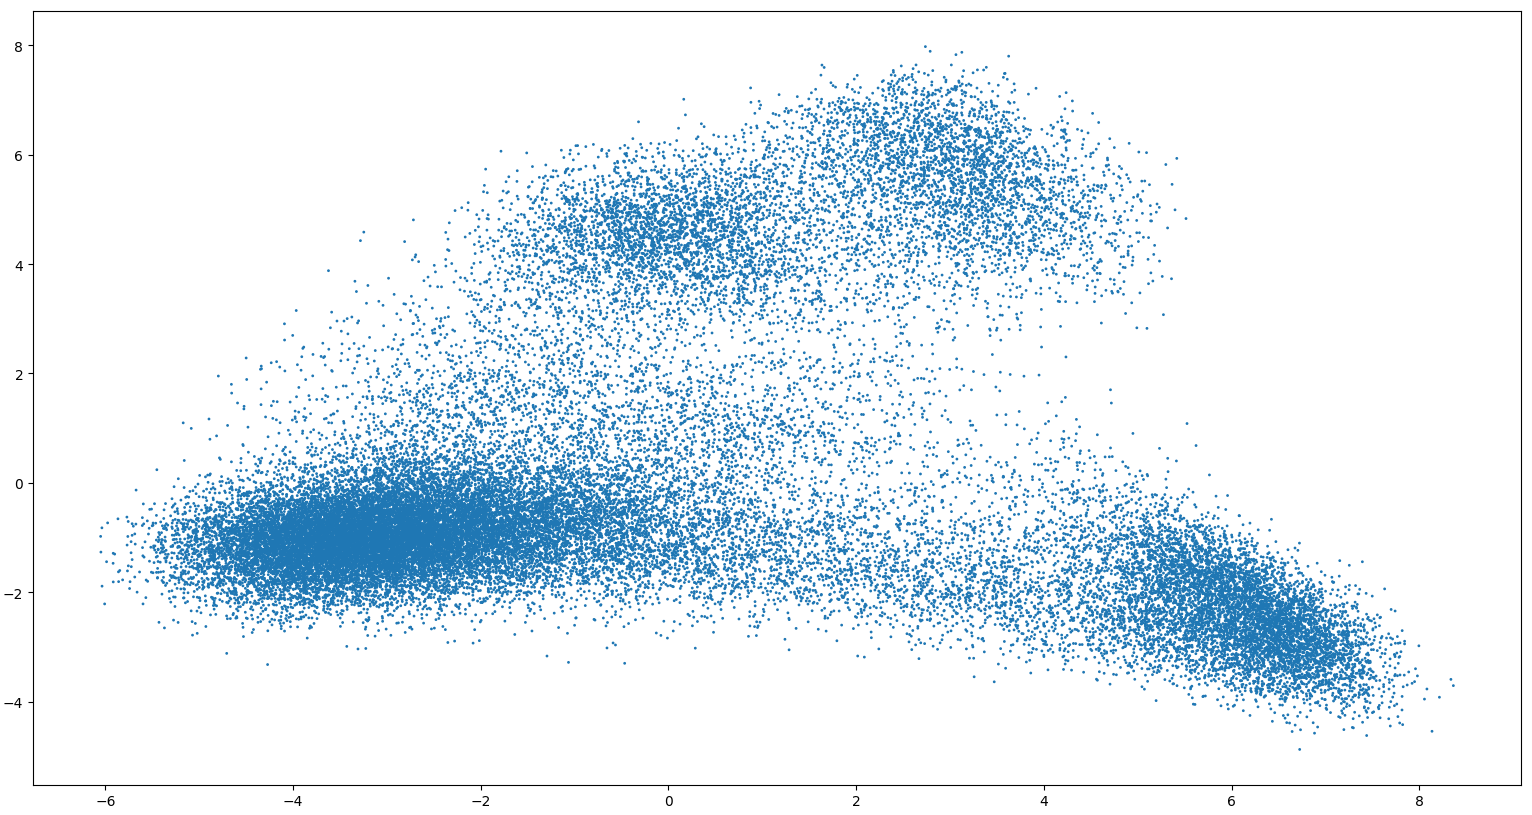
\includegraphics[width=0.45\textwidth]{img/plant.png}
    \caption{2D PCA projection of the state cloud associated with the symbol "plant"}\label{fig:plant}
\end{figure}

\begin{table}[!bp]
    \caption{Context samples by K-means cluster of "plant" state cloud.}
    \label{tab:samples}
    \begin{tabular}{|l|l|}
        \hline
        \textbf{Cluster} & \textbf{Sample context} \\
        \hline
        1 & \parbox{0.7\linewidth}{absently, i raised the blinds so that the plant was able to soak in the
        impromptu sunshine.} \\
        \hline
        & \parbox{0.7\linewidth}{i’ve brought you over a few macramé plant hangers to decorate your room.} \\
        \hline
        2 & \parbox{0.7\linewidth}{i wanted to plant them myself.} \\
        \hline
         & \parbox{0.7\linewidth}{she’ll just plant new ones and start all over again.} \\
        \hline
        3 & \parbox{0.7\linewidth}{the computers running the plant were all infected, of course.} \\
        \hline
        & \parbox{0.7\linewidth}{it was plant shutdown for two weeks.} \\
        \hline
    \end{tabular}
\end{table}

This diversity of meanings assumed by the same symbol across the text corpus casts doubt on our assumption of there being a one-to-one correspondence between symbols and graph nodes. An intermediate clustering step might be effective in decoupling different word senses and producing different state clouds, though the issue of how many senses are there per symbol is non-trivial. Similar to how words themselves appear to discretely quantize the otherwise continuous semantic space, finite word senses as "subsymbols" run into similar trade-offs between sparsity and accuracy.

\subsubsection{State clouds are non-linear.}

While we employ conceptors as compact elliptical objects which approximate high-dimensional state clouds of contextual embeddings, their limited expressivity might fail to capture the intricate non-linear layout of real-world embeddings. Low-dimensional PCA projections of several state clouds of BERT embeddings radically diverge from Gaussian distributions, bringing into question the suitability of elliptical conceptors to represent them (see Fig. \ref{fig:earth}). However, we note that state clouds of less ambiguous terms (i.e. limited number of word senses) appear more well-formed. Non-linearities might arise mainly from diverse word senses being assumed by the same symbols.

\begin{figure}[h]
    \centering
    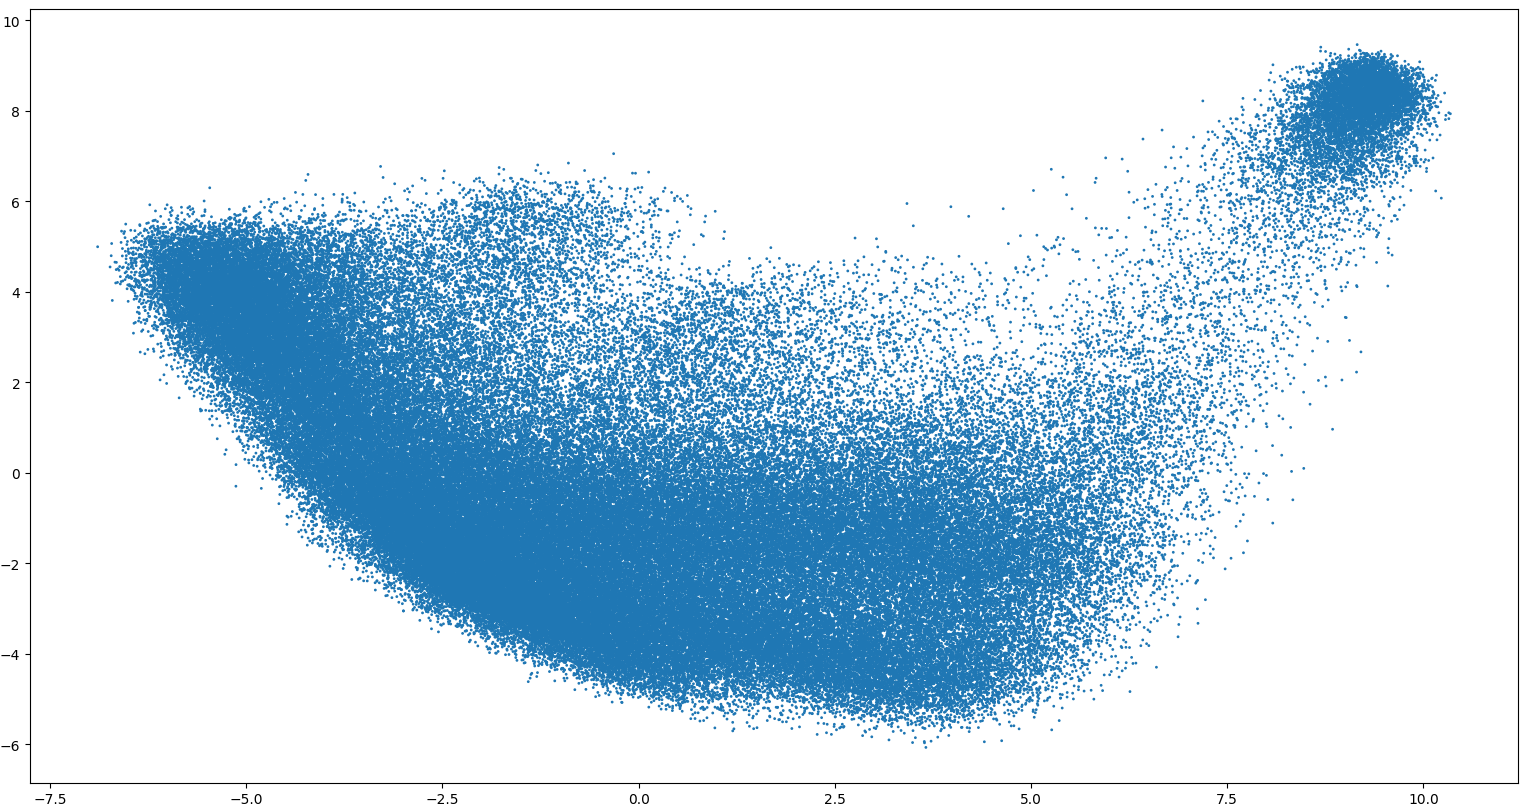
\includegraphics[width=0.45\textwidth]{img/earth.png}
    \caption{2D PCA projection of the state cloud associated with the symbol "earth"}\label{fig:earth}
\end{figure}

\subsubsection{NSC requires many exemplars.}

The central role of state clouds in NSC means that the technique is highly dependent on a large number of occurences and contexts for each concept analyzed. This makes it difficult to interpret the model's internal representations with respect to obscure tokens, as those are extremely rare in natural datasets. However, synthetic datasets might address this issue, provided the ability to synthesize a wide range of unique contexts for an arbitrary concept.

\subsubsection{NSC output graph is heavily influenced by the graph search objective.}

The graph search process employed to output a knowledge graph is highly sensitive to the search objective. Reaching a balance between the functional-grounded terms (e.g. faithfulness to detected abstraction ordering) and human-grounded terms (e.g. sparsity) is difficult to achieve manually. Often, one component of the linear combination tends dominates the others (see Fig. \ref{fig:children} and Fig. \ref{fig:pruning}). This balance is especially difficult to find with higher number of concepts, bringing the scalability of NSC into question. However, normalizing the objective's components based on the number of concepts being analyzed greatly improved robustness.

\begin{figure}[h]
\centering
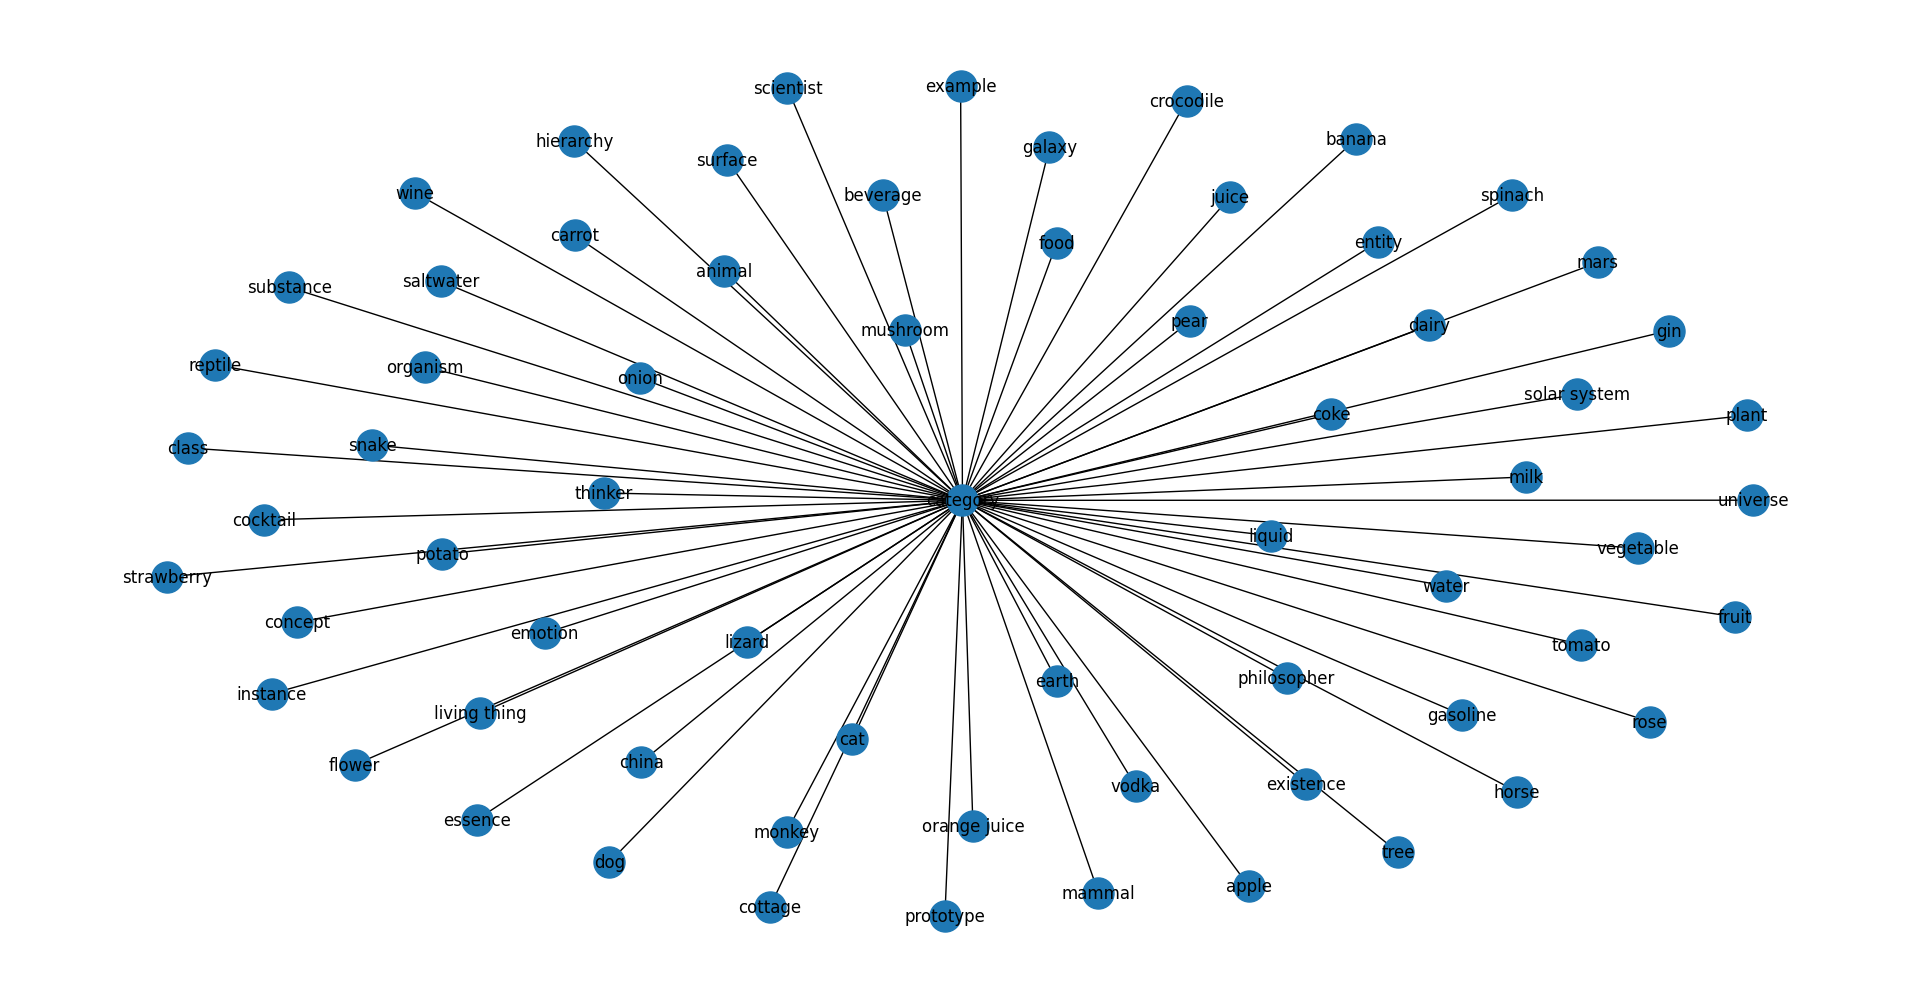
\includegraphics[width=0.45\textwidth]{img/too_much_pruning.png}
\caption{NSC output graph after undervaluing children count per node constraints.}\label{fig:children}
\end{figure}

\begin{figure}[h]
\centering
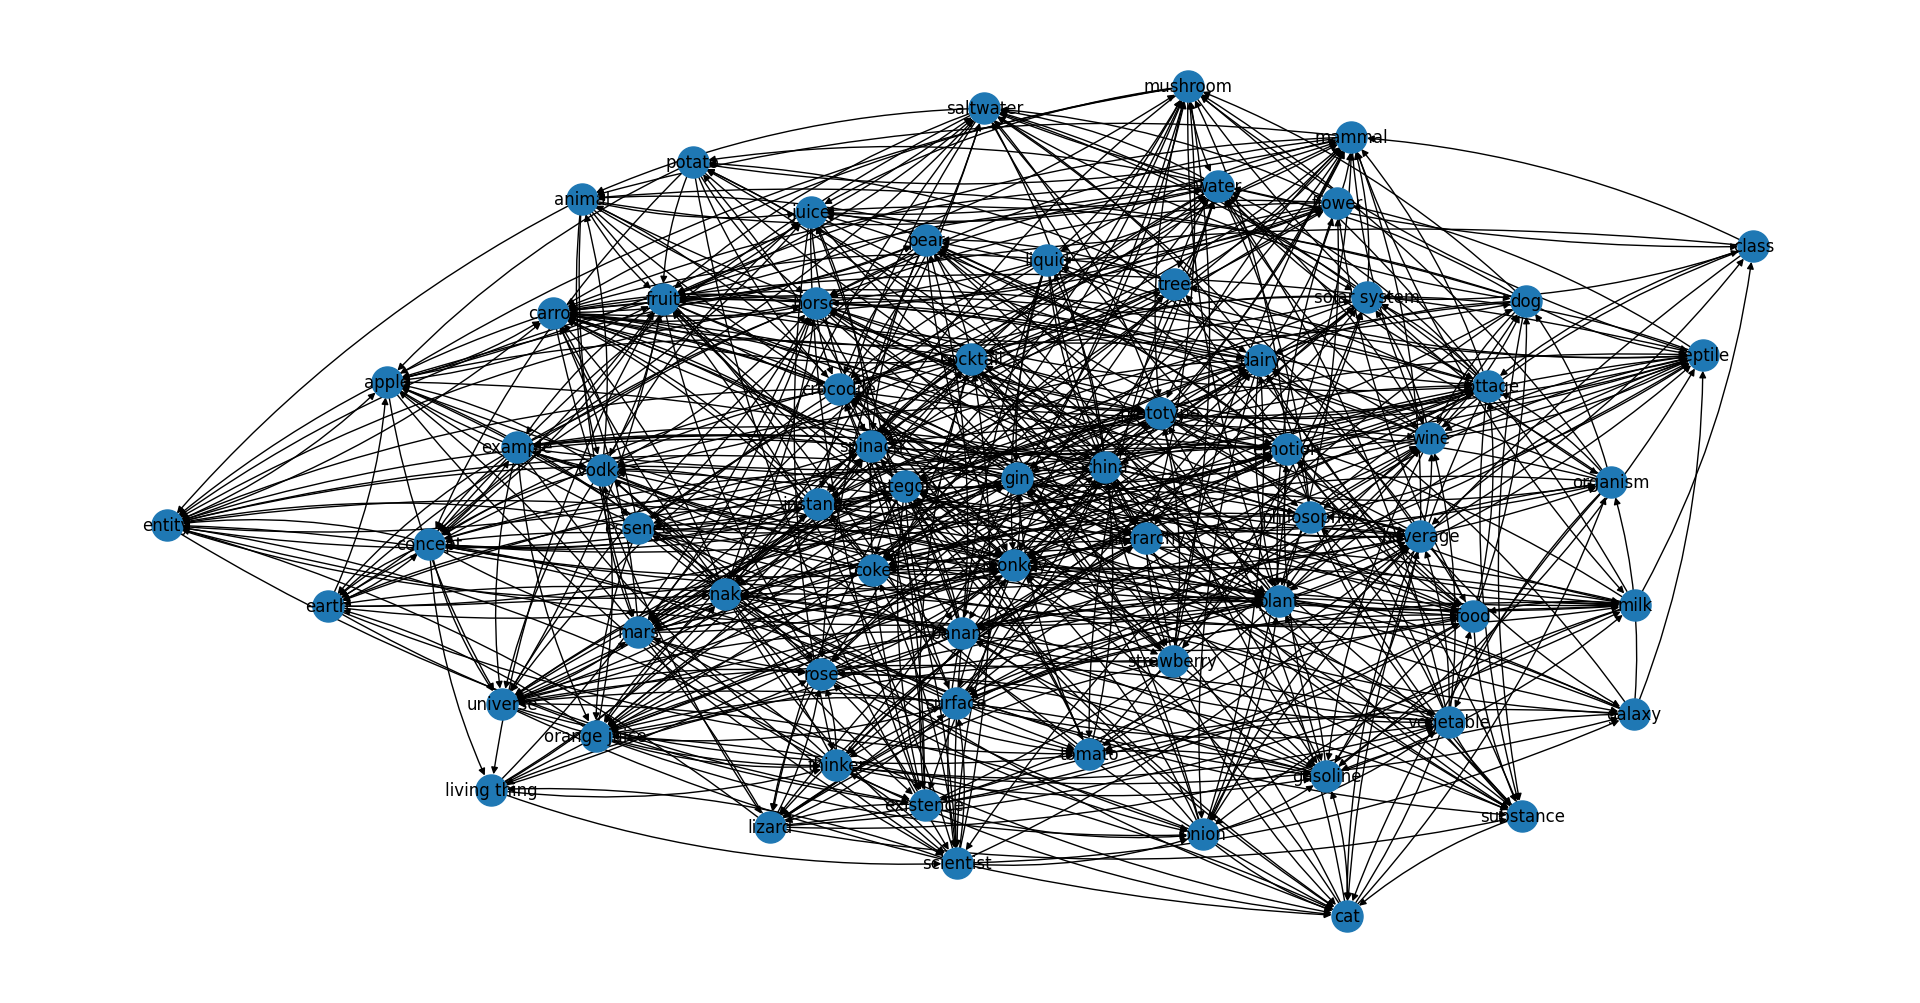
\includegraphics[width=0.45\textwidth]{img/short_run.png}
\caption{NSC output graph after undervaluing arc pruning.}\label{fig:pruning}
\end{figure}

\subsection{Future work}

\subsubsection{Non-linear conceptors}

Non-linear variations of classical conceptors might be used to capture the internal structure of high-dimensional state clouds of contextual embeddings better than the original elliptical objects. It had been suggested that shallow MLPs could be employed for this task, yet this brings additional questions of interpretability. As we attempt to model high-dimensional representations ever more accurately, we might be forced to depart from sparse human-grounded explanations.

\subsubsection{Beyond abstraction}

While this work focuses solely on the meronymous IS\_A relationship of abstraction between to concepts, it's conceivable that the difference matrix computed in NSC as an intermediate step contains a rich representation of other relationships between concepts. This is reminiscent of the seemingly algebraic properties of prototype word embeddings (e.g. "king" + "woman" - "man" ~ "queen"), which appear to encode diverse analogies and conceptual relationships. The relative spatial layout of entire state clouds might provide similar information, yet richer.
